% WORKING DRAFT FOR BOTH AUTHORS TO REVIEW, EDIT AND APPROVE.
% Uses the supplied F26 template support files unchanged.
% Numerical sources: repo commit 9f83e01ec1d940e6255bd801c7559434c0b8e6ef;
% Rahil's regional and test values: transferred MSI archives, Nov. 24, 2026.
% Confirm names/emails, contribution statements and assistance disclosure.
% Replace draft wording with explanations you understand and can defend.
\documentclass{article}
\usepackage[T1]{fontenc}
\usepackage{style,times}
\usepackage{hyperref}
\usepackage{url}
\usepackage{wrapfig,graphicx}
\usepackage{amsmath}

\title{Reducing Ghosting in HDR Images}
\lhead{EE5561 - F26 - Project Intermediate Report}
\rhead{November 24, 2026}
\author{Rahil Sheth, Zijian Zhang \\
Team HDR \\
\texttt{sheth047@umn.edu, zha00175@umn.edu}}
\newcommand{\fix}{\marginpar{FIX}}
\newcommand{\new}{\marginpar{NEW}}
\finalcopy
\begin{document}
\maketitle

\begin{abstract}
Movement between bracketed exposures can produce ghosts in an HDR merge. We test exposure and alignment-reliability cues for choosing original versus aligned features. Four variants share a training-update budget, with checkpoints selected on five validation scenes. On 15 separate test entries, the gate with constant cues reaches 43.302 dB PSNR-mu and measured cues reach 43.388 dB. This small gain varies by scene and is strongly influenced by one case. We report the split, controls, visual failures, and remaining tests.
\end{abstract}

\section{Introduction}
High dynamic range (HDR) imaging preserves detail across bright and dark areas. We merge photos taken at different exposures to recover that range. Ghosting happens when something moves from shot to shot. When those photos are merged, we can get double edges and see-through copies of objects. Rahil suggested this project because he is interested in photography and has run into this problem while shooting. Our goal is to remove those ghosts while keeping the detail that made us take an HDR bracket in the first place.

We use the middle exposure as the reference pose and coordinate system. Using only that image avoids merging different poses, but loses detail where it is clipped. Alignment can recover useful information from the other photos and can also introduce errors. We test whether explicit exposure and alignment-reliability cues help a learned gate choose between original and aligned features. Comparing the same gate with constant versus measured cues separates their effect from the extra feature path.

\section{Related Works}
\citet{kalantari2017} provide the dynamic-scene HDR dataset used here and study learning-based merging. AHDRNet uses the reference to weight non-reference features before merging, with dilated residual dense blocks providing wider context \citep{yan2019}. Our backbone follows that approach.

FlexHDR explicitly models exposure and alignment uncertainties \citep{catley2022}. SAFNet selectively combines alignment and fusion and provides a harder captured dataset \citep{kong2024}. Our work implements an original/aligned feature gate and controls for testing the added cues. Reliability-aware fusion is therefore prior work; the contribution here is the implementation and controlled comparison.

\section{Methodology}
\subsection{Dataset and exposure conversion}
The Kalantari training archive contains 74 scenes, each with three $1500\times1000$ RGB TIFFs and an HDR target. We keep 69 scenes for training and \texttt{025, 045, 051, 056, 062} for validation. A thumbnail normalized-correlation check at 0.9 identifies 16 related-scene groups; none cross this split. Crops and flips/rotations are sampled from training scenes only. Validation uses full images and does not update weights.

The separate test archive has five PAPER and ten EXTRA entries. Checkpoint hashes, preprocessing, and metrics were frozen before evaluation. Input-file hashes and reference thumbnails checked against all 74 Training scenes produced no overlap or correlation flags; undetected relatives remain possible. Two test pairs share identical reference/target files: EXTRA/003 with LadySitting, and EXTRA/005 with PeopleStanding. We retain all 15 published entries in the primary average, but they are not 15 independent capture conditions.

\begin{table}[t]
\centering
\small
\begin{tabular}{lrl}
\hline
Partition & Entries & Purpose \\
\hline
Training & 69 & Learn weights from random crops \\
Validation & 5 & Select checkpoints; inspect development failures \\
Separate test & 15 & Score frozen models; no further tuning \\
\hline
\end{tabular}
\caption{Scene-level separation. Every crop from a scene stays in its partition. Test entries come from the separate archive.}
\label{tab:split}
\end{table}

For uint16 RGB values, we compute
\begin{equation}
L_i=I_i/65535,\qquad t_i=2^{e_i},\qquad H_i=L_i^{2.2}/t_i,\qquad X_i=[L_i,H_i].
\end{equation}
$e_i$ comes from \texttt{exposure.txt}; $t_i$ is relative time, not seconds. Gamma 2.2 follows the dataset pipeline. Dividing by exposure puts usable measurements on a common radiance scale, but cannot undo clipping. Each $X_i$ has three stored-image and three radiance channels. No target-fitted scaling is used.

\subsection{Classical controls and alignment}
C0 uses the middle-exposure radiance $H_2$ alone. C1 combines all exposures using a triangular weight $w_i=1-|2L_i-1|$ and the weighted average $\widehat H=\sum_i w_iH_i/\sum_i w_i$. Each color channel receives the most weight near the middle of its stored intensity range, avoiding very dark or clipped measurements.

C2 reduces a non-reference contribution when it disagrees with a usable reference channel. Specifically, if $0.1\leq L_2\leq0.9$ and
\begin{equation}
|H_i-H_2|/\max(H_i,H_2,10^{-4})>0.25,
\end{equation}
its weight becomes zero. Other contributions remain in the weighted merge. C3 applies the same rule after optical-flow alignment, with non-reference weights also multiplied by an in-bounds validity mask. If the total weight is below $10^{-3}$, the code chooses the shortest exposure when $\max_{RGB}L_2\geq0.5$, otherwise the longest; an invalid sample falls back to the reference. These controls use a specified weighted merge, rather than a full camera-response-calibrated HDR method.

Optical flow estimates where a pixel in the reference should be sampled in another image. Warping uses those locations to resample the source. We use OpenCV's medium-preset DIS flow \citep{kroeger2016}. Before flow estimation, the darker photo is raised to the brighter photo's exposure using the same gamma/exposure model. The estimated flow then warps the original source image. A synthetic translation check verifies the sampling direction and invalid borders; it is a code diagnostic, not a camera-shake benchmark.

\subsection{Backbone and original/aligned gate}
The AHDRNet-style encoder maps each six-channel input to 64 features using a $3\times3$ convolution and LeakyReLU. For each non-reference exposure, attention concatenates its features with the reference features, applies two $3\times3$ convolutions and a sigmoid, and produces a $64\times H\times W$ mask. This mask weights non-reference features across position and channel before merging.

The merge network has three dilated residual dense blocks. Each contains six dense layers with growth 32 and dilation 2. Dilation widens context without reducing resolution. Dense connections retain earlier features; residual connections provide a path around a block. Our added gate chooses original versus aligned features before this backbone merges them.

\begin{figure}[t]
\centering
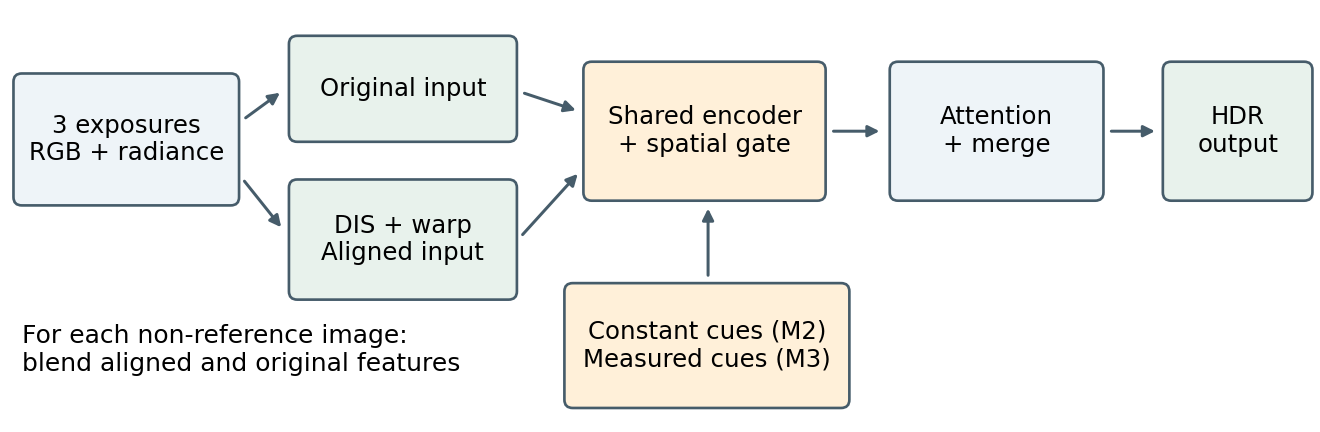
\includegraphics[width=\linewidth]{figures/pipeline.png}
\caption{Implemented M2/M3 paths with a shared encoder and hard warp-validity mask. M2 uses constant cue channels; M3 uses measured exposure and flow-consistency cues. This is an architecture schematic.}
\label{fig:pipeline}
\end{figure}

M0 uses original inputs; M1 tests alignment with the same backbone. M2 adds both paths and a gate; M3 tests measured cues against M2 at equal capacity (Fig.~\ref{fig:pipeline}). The gate uses reference, original, and aligned features:
\begin{equation}
g_i=v_i\sigma\!\left(G_i([Z_2,Z_i^o,Z_i^w,c_i])\right),\qquad
\widetilde Z_i=g_iZ_i^w+(1-g_i)Z_i^o.
\end{equation}
Values near one favor aligned features; values near zero favor original features. $G_i$ uses two $3\times3$ convolutions with $196\!\rightarrow\!64\!\rightarrow\!1$ channels. $v_i$ is zero when the sampling location is outside the source, forcing the original path at that pixel.

M2 sets all four cue channels to one. M3 uses $c_i=[q_2,q_i^w,v_i,r_i]$, where $q(L)=1-|2\max_{RGB}(L)-1|$ measures distance from extreme brightness and $r_i=\exp(-E_i/2)$ measures forward/backward flow agreement. $E_i$ is the squared disagreement after resampling the backward flow. These estimated cues are not motion labels. Both retain hard validity $v_i$ and equal parameter counts. M3 versus M2 tests cue inputs; M2 versus M1 also changes architecture and capacity.

\subsection{Training, compute, and evaluation}
Pilots ran on MSI A100-SXM4-40GB GPUs through Slurm (Python 3.11.13, PyTorch 2.7.1+cu126, CUDA 12.6, OpenCV 5.1.0). Rahil verified GPU updates and ran test evaluation in MSI OnDemand with PyTorch 2.7.1+cu118, CUDA 11.8, and OpenCV 4.10.0. The implementation is frozen, but runtime versions differ. Each used seed 5561, Adam with $(0.9,0.999)$, learning rate $10^{-4}$, batch eight, $256\times256$ crops, flips and 90-degree rotations, and 50,000 updates. Training used FP32 with TF32 disabled. M0/M1 have 1,441,283 parameters; M2/M3 have 1,668,357. Equal update counts do not imply equal compute cost.

The loss is mean absolute error after the mapping
\begin{equation}
T(H)=\frac{\log(1+5000\operatorname{clip}(H,0,1))}{\log(5001)}.
\end{equation}
This compresses radiance before measuring error. Validation scores the full images every 2,000 updates, with no border removed. PSNR uses peak one; SSIM uses a uniform $7\times7$ window, sample covariance, and RGB averaging. Linear scores use clipped radiance; mu-domain scores use $T$. Each model selects its best mean validation PSNR-mu checkpoint within the common budget; all select update 50,000. Test inference uses evaluation mode without gradients or an optimizer. All 120 method/scene pairs were completed in 271 s; test targets enter metrics, not checkpoint selection. Comparisons use the same runtime within each partition.

\section{Results}
\subsection{Controls and validation}
Table~\ref{tab:results} reports equal-entry means under the specified metrics. On validation, C3 exceeds reference only by 2.62 dB PSNR-mu, but loses on some scenes. M1 exceeds M0 by 0.76 dB; M2 exceeds M1 by 0.91 dB, including the added path, gate, and parameters. M3 is 0.043 dB below M2. The direct cue control therefore shows no validation PSNR gain.

\begin{table}[t]
\centering
\small
\begin{tabular}{llrrr}
\hline
 & Method & Val. PSNR-mu & Test PSNR-mu & Test SSIM-mu \\
\hline
C0 & Reference only & 36.59 & 38.189 & 0.97527 \\
C1 & Weighted merge & 22.51 & 24.901 & 0.83055 \\
C2 & Channel-wise rejection & 26.84 & 28.315 & 0.92284 \\
C3 & Aligned rejection & 39.21 & 35.087 & 0.96903 \\
M0 & Original inputs & 42.46 & 42.903 & 0.98957 \\
M1 & Aligned inputs & 43.22 & 42.821 & 0.99036 \\
M2 & Dual path, constant cues & 44.13 & 43.302 & 0.99046 \\
M3 & Dual path, measured cues & 44.09 & 43.388 & 0.99052 \\
\hline
\end{tabular}
\caption{Five validation scenes and all 15 test entries; PSNR in dB. M0--M3 use one seed, 50,000 updates, and validation-selected checkpoints. All methods use the same runtime within each partition.}
\label{tab:results}
\end{table}

\begin{figure}[t]
\centering
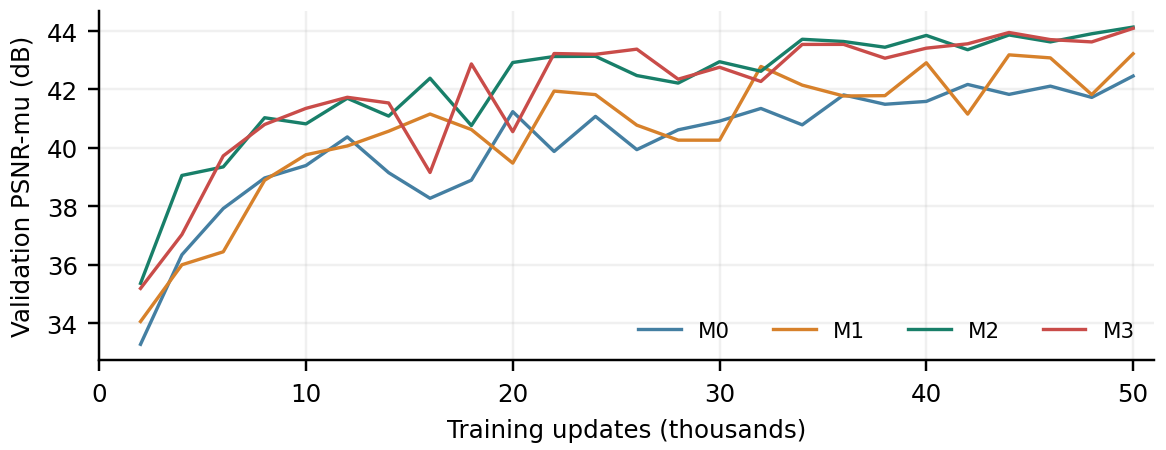
\includegraphics[width=0.84\linewidth]{figures/fig_variants_curve.png}
\caption{Saved mean validation PSNR-mu. M2/M3 remain close, and scores still fluctuate at 50,000 updates; convergence is not established.}
\label{fig:learning}
\end{figure}

Pilot wall times including evaluation were 6.20, 6.39, 7.05, and 7.10 hours. Fitting four training crops for 3,000 updates reached 43.45 dB for M0 and 43.75 dB for M3, versus C0's 36.96 dB. These are fitting checks. Repeated M0 validation gave matching metrics and bit-identical outputs.

\subsection{Frozen test evaluation}
On all 15 entries, M3 exceeds M2 by 0.0856 dB PSNR-mu and wins on nine entries, losing on six. The mean gain is +0.245 dB on PAPER and +0.006 dB on EXTRA. ManStanding contributes +1.261 dB. As a post-hoc sensitivity check, the other 14 entries average only +0.0017 dB. All 15 remain in the primary result. One seed and correlated test entries do not establish a reliable general cue advantage.



Alignment is not uniformly beneficial: test C3 scores 35.09 dB versus reference only at 38.19 dB, and M1 is 0.082 dB below M0. These are within-test comparisons. Changes from validation cannot be attributed solely to the data because runtime versions also differ.

Fig.~\ref{fig:test-case} uses an input-selected face crop fixed before test evaluation. The merge doubles the face; C3 distorts boundaries. Learned outputs remove the large duplication but look similar, without a clear visible M3 advantage. Outputs/target share one reference-derived Reinhard exposure and gamma display. Scores use float outputs and the fixed mu mapping.

\begin{figure}[t]
\centering
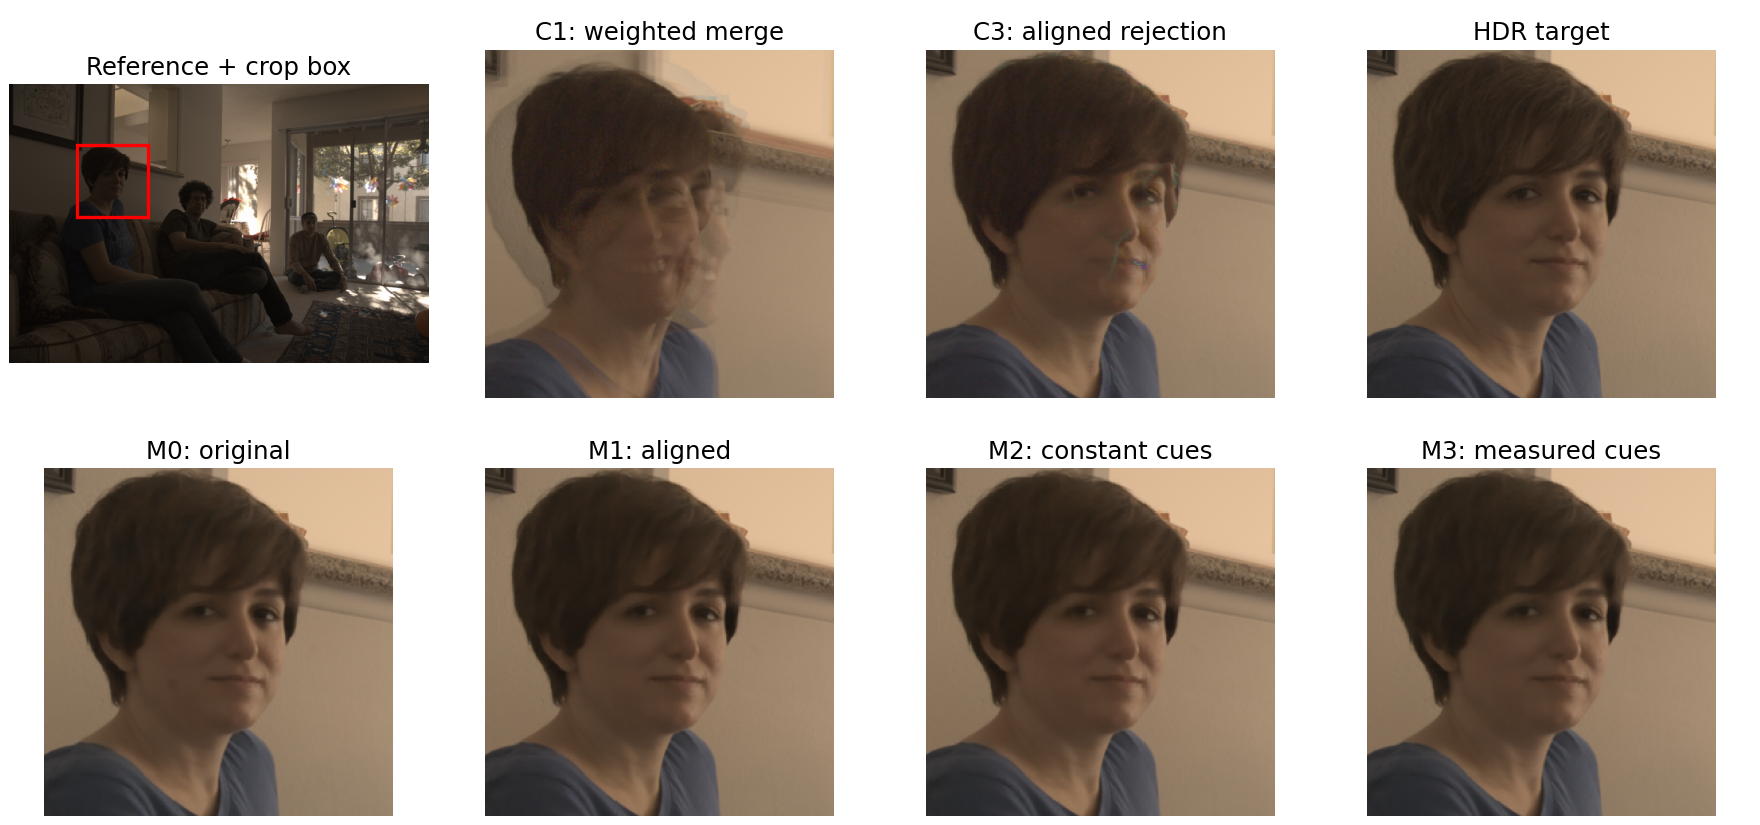
\includegraphics[width=\linewidth]{figures/test_people_talking.png}
\caption{PeopleTalking test case, crop $(240,220,256,256)$. The red box locates the patch. C1 doubles the face; C3 leaves artifacts near the facial boundary. M0--M3 differences are subtle. The dataset target is the desired reconstruction. Only the locator uses stored LDR encoding.}
\label{fig:test-case}
\end{figure}

\subsection{Development failure analysis}
Rahil re-scored the frozen M0--M3 predictions on the five validation scenes; all 20 full-image PSNR/SSIM pairs match the saved records. His separate whole-pixel fallback replaces the weighted merge with reference only when every reference channel is in $(0.05,0.95)$ and either source is outside that range or has $\max_{RGB}|H_i-H_2|/(H_i+H_2+10^{-6})>0.20$. Otherwise it keeps the merge. This differs from C2. Its mean PSNR-mu is 30.36 dB, versus 22.51 dB for his merge and 36.59 dB for reference only.

Input-defined bright regions have any reference channel at least 0.95; usable regions have all channels in $(0.05,0.95)$. These are brightness proxies, not verified motion or clipping. M3 lowers bright-region mu-MAE only in validation scene 062 (7.84\%); it raises that error in the other four scenes. Scene 045 has only 24 bright pixels, so its regional result has very limited coverage. This exploratory analysis reuses model-selection scenes; SSIM is scored only on full images.

\section{Discussion and Next Steps}
Measured cues give a small, uneven benefit, motivating separate exposure-cue and flow-cue ablations. The Kalantari holdout does not resolve the concern about limited motion diversity.

Following feedback, we shifted from the proposed synthetic-motion benchmark and method selector to captured-scene controls and the cue comparison. We specify classical rules, gamma, attention, dilation, and the gate; synthetic shifts check code only. We checked an interrupted download, moved large files after quota limits, and grouped detected relatives before training.

Next, Zijian will run individual-cue ablations and additional seeds. Rahil will audit Challenge123's exposure/target conventions and annotate motion/clipping cases for external evaluation \citep{kong2024}. Camera-shake and cross-dataset tests remain uncompleted. The current test results will not be used to retune these reported checkpoints.

\subsubsection*{Work Done by Each Member}
% AUTHOR REVIEW REQUIRED: these statements describe observed work, not the R/Z folder labels.
\textbf{Rahil Sheth:} proposed the photography problem; checked his MSI GPU environment; downloaded and inventoried the data; inspected scene 001; ran classical controls and regional analysis on five validation scenes, checked 20 saved model-score pairs, and ran the frozen 15-entry test evaluation with overlap checks and diagnostic figures.

\textbf{Zijian Zhang:} implemented the shared data/model pipeline, alignment, and gate; ran fitting checks and four model pilots; and organized evaluation records, checkpoints, and figures.

% Confirm assistance disclosure with both authors/course policy.
\textbf{Assistance:} AI supported setup/evaluation scripts, repository checks, figures, and drafting. Metrics come from recorded experiments.

\clearpage
\bibliography{refs}
\bibliographystyle{refs}
\end{document}
